\section{Architecture} 
\label{sec:design}

We design CodFS, an erasure-coded clustered storage system that implements 
the aforementioned delta-based update schemes to support efficient updates 
and recovery.  

%CodFS follows the typical single-master-multiple-slave distributed system
%design as shown in 
Figure~\ref{fig:architecture} shows the CodFS architecture.  The
{\em metadata server (MDS)} stores and manages all file metadata, while
multiple {\em object storage devices (OSDs)} perform coding operations and
store the data and parity chunks.  The MDS also plays a monitor role, such
that it keeps track of the health status of the OSDs and triggers recovery
when some OSDs fail.  A CodFS client can access the storage cluster through a
file system interface. 

\section{Work Flow}
\label{sec:workflow}

\subsection{Normal Operations}

CodFS performs erasure coding on the write path as illustrated in
Figure~\ref{fig:architecture}.  To write a file, the client first splits the
file into segments, and requests the MDS to store the metadata and identify
the {\em primary OSD} for each segment.  The client then sends each segment to
its primary OSD, which encodes the segment into $k$ data chunks and $n-k$
parity chunks for some pre-specified parameters $n$ and $k$.  The primary OSD
stores a data chunk locally, and distributes the remaining $n-1$ chunks to
other OSDs called the {\em secondary OSDs} for the segment.  The identities of
the secondary OSDs are assigned by the MDS to keep the entire cluster
load-balanced.  Both primary and secondary OSDs are defined in a logical
sense, such that each physical OSD can act as a primary OSD for some segments
and a secondary OSD for others. 

\begin{figure}[t]
    \centering
    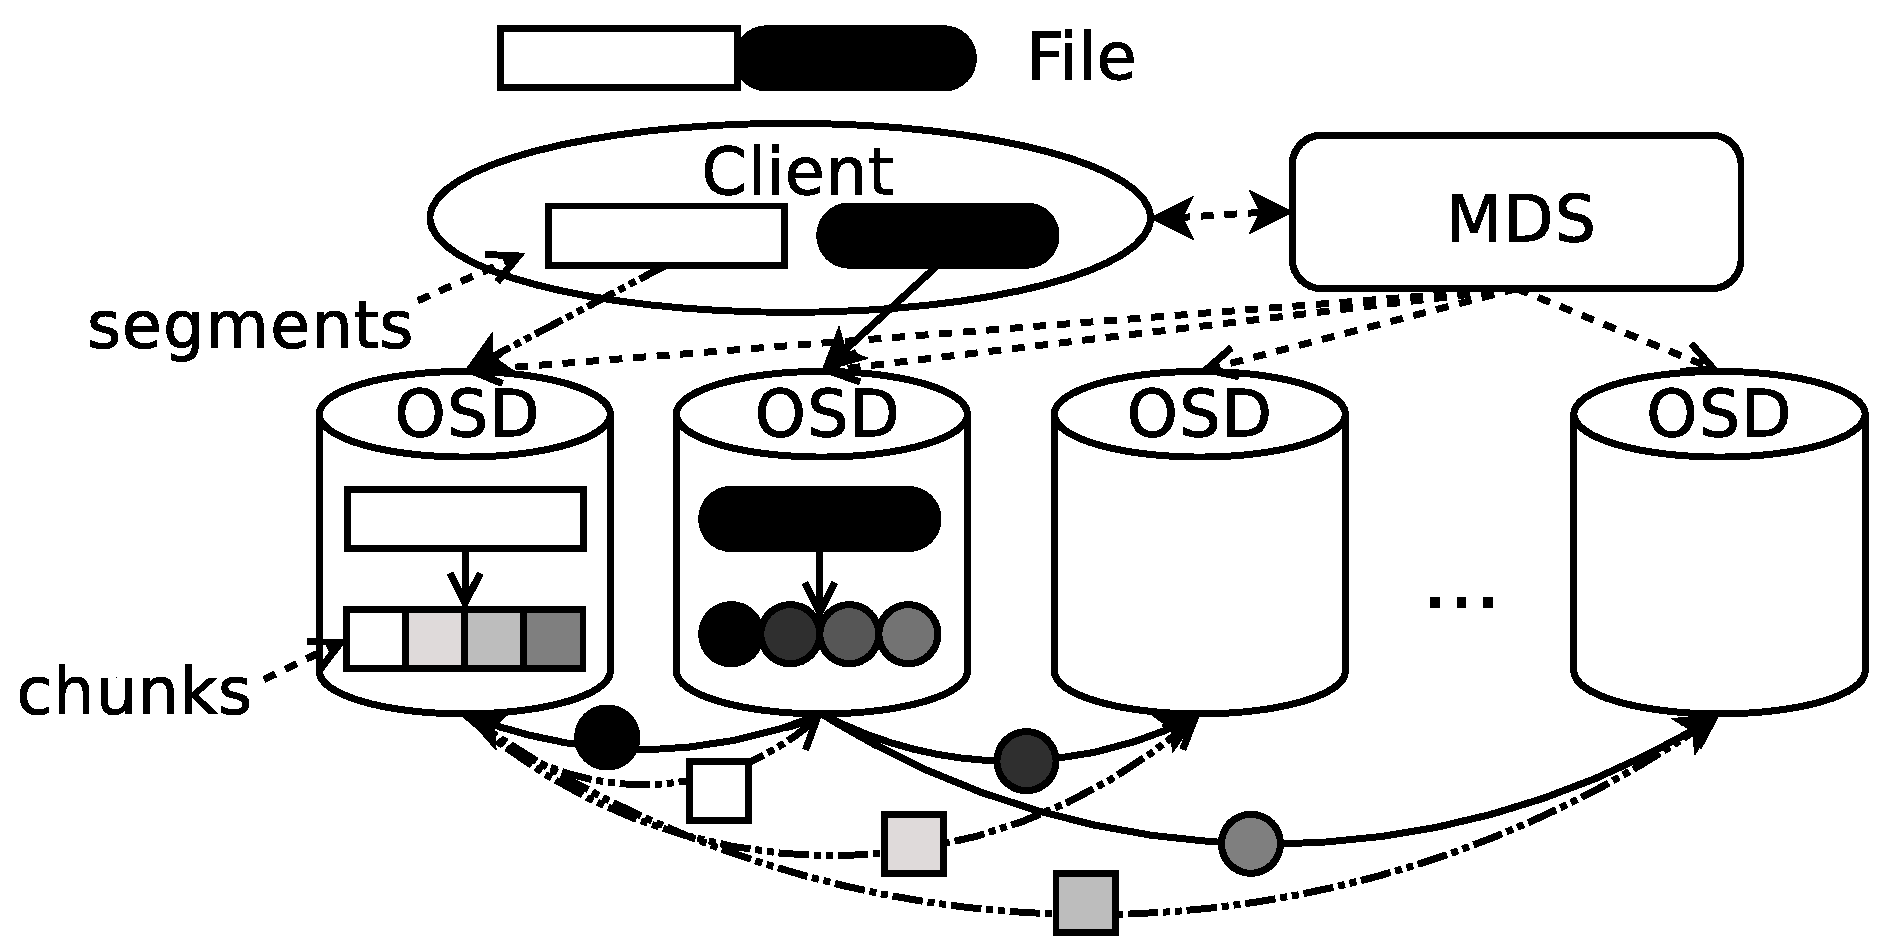
\includegraphics[width=0.7\linewidth]{figs/architecture}
    \caption{CodFS architecture.} %: A client divides data into segments and sends
	%them to different primary OSDs, each of which further encodes a segment
	%into chunks and sends them to secondary OSDs.}
    \label{fig:architecture}
\end{figure}

To read a segment, the client first queries MDS for the primary OSD.  It then
issues a read request to the primary OSD, which collects one data chunk
locally and $k-1$ data chunks from other secondary OSDs and returns the
original segment to the client. In the normal state where no failure occurs,
the primary OSD only needs the $k$ data chunks of the segment for rebuilding. 

CodFS adopts the delta-based approach for data updates.  
%and supports all the four approaches described in
%\S\ref{sec:delta_based}. 
To update a segment, the client sends the modified data with the corresponding offsets
to the segment's primary OSD, which 
first splits the update into sub-updates according to the offsets, 
such that each sub-update targets a single data chunk. The primary OSD then 
sends each sub-update to the OSD storing the targeted data chunk.
Upon receiving a sub-update for a data chunk, an OSD computes the parity
deltas and distributes them to the parity destinations. Finally, both the updates and 
parity deltas are saved according to the chosen update scheme.

\subsection{Degraded Operations}

CodFS switches to degraded mode when some OSDs fail (assuming the number of
failed OSDs is tolerable). 
% if the number of failed OSDs is within the tolerable level of the erasure
% coding applied to the segment, 
The primary OSD coordinates the degraded operations for its responsible
segments.  If the primary OSD of a segment fails, CodFS promotes another
surviving secondary OSD of the segment to be the primary OSD.  CodFS supports
degraded reads and recovery.  To issue a degraded read to a segment, the
primary OSD follows the same read path as the normal case, except that it
collects both data and parity chunks of the segment.  It then decodes the
collected chunks and returns the original segment.  If an OSD failure is
deemed permanent, CodFS can recover the lost chunks on a new OSD.  That is,
for each segment with lost chunks, the corresponding primary OSD first
reconstructs the segment as in degraded reads, and then writes the lost chunk
to the new OSD.   Our current implementation of degraded reads and recovery
uses the standard approach that reads $k$ chunks for reconstruction, and it
works for any number of failed OSDs no more than $n-k$.  Nevertheless, our
design is also compatible with efficient recovery approaches that read less
data under single failures (e.g., \cite{xiang10,khan12}). 

%\paragraph{Degraded-write} For degraded write, CodFS follows the normal write
%procedure and the failure-tolerance is still guaranteed unless the number of
%alive OSDs is less then the number of coded chunk. 

%\paragraph{Degraded-update} CodFS uses primary OSD to send data updates to
%the OSDs that contain the data chunks to be updated. So if the target OSD for
%an update is still alive, CodFS follows the normal update flow. Otherwise,
%CodFS first triggers the recovery procedure for the segment and recovery
%the lost data chunk in another OSD and then follow the normal procedure.

%The recovery process first look up the MDS to find out the segments that need
%to be recovered. For each segment, CodFS first switches the primary OSD if
%the original one fails.  Then the primary OSD first performs a degraded read
%of the segment and computes the lost chunks. The lost chunks are then
%distributed to new secondary OSDs which are selected by the MDS.

%The MDS detects OSD failures and triggers recovery process in CodFS. The
%recovery process can be triggered either manually or automatically. For
%automatic recovery, we set a delay to trigger recovery after detecting OSD
%failures to avoid generating useless recovery traffic caused by transient
%failure such as network partition. 

\section{Implementation Issues}
\label{sec:issues}

We address several implementation issues in CodFS and justify our design
choices. 

\subsection{Consistency} CodFS provides close-to-open consistency
\cite{howard88}, which offers the same level of consistency as most Network
File Systems (NFS) clients. Any open request to a segment always
returns the version following the previous close request. CodFS directs all
reads and writes of a segment through the corresponding primary OSD, which
uses a lock-based approach to serialize the requests of all clients.  This
simplifies consistency implementation. 

\subsection{Offloading} 
%The primary OSD not only simplifies consistency implementation, but also 
CodFS offloads the encoding and reconstruction operations from clients. 
Client-side encoding generates more write traffic 
%to the storage cluster 
since the client needs to transmit parity chunks.  Using the primary
OSD design limits the fan-outs of clients and the traffic between the
clients and the storage cluster.  In addition, CodFS splits each file into
segments, which are handled by different primary OSDs in parallel.  Hence, the
computational power of a single OSD will not become a bottleneck on the write
path.  Also, within each OSD, CodFS uses multi-threading to pipeline and
parallelize the I/O and encoding operations, so as to mitigate the overhead
in encoding computations. 
%We validate this in \S\ref{sec:evaluation_baseline}.
%We show that the theoretical read/write throughput of such design is bounded
%by the network bandwidth and we prove that CodFS can reach the theoretical
%bound in \S\ref{sec:evaluation_baseline}.
%\red{addressed network bound}

\subsection{Metadata Management} The MDS stores all metadata in a
key-value database built on MongoDB~\cite{mongodb}. CodFS can configure a
backup MDS to serve the metadata operations in case the main MDS fails,
similar to HDFS~\cite{hdfs_architecture}. 
%which is replicated to avoid metadata loss. 
%that is replicated which enables replication backups to avoid the loss of
%metadata when the MDS fails. 

\subsection{Caching} CodFS adopts simple caching techniques to boost the entire
system performance.  Each CodFS client is equipped with an LRU cache for
segments so that frequent updates of a single segment can be batched and sent
to the primary OSD. 
% which reduces the network round trip time.
The LRU cache also favors frequent reads of a single segment, to avoid
fetching the segment from the storage cluster in each read.  We do not
consider specific write mitigation techniques (e.g., lazy write-back and
compression) or advanced caches (e.g., distributed caching or SSDs), although
our system can be extended with such approaches. 

%Both the clients and MDS contains a metadata cache module. For clients, the
%metadata cache can reduce the round-trip to the MDS, while for MDS, the cache
%module can reduce frequent queries made to the database.

\subsection{Segment Size} CodFS supports flexible segment size from
16MB to 64MB and sets the default at 16MB. This size is chosen to fully
utilize both the network bandwidth and disk throughput, as shown in our 
experiments (see \S\ref{sec:evaluation_baseline}). Smaller segments
lead to more disk I/Os and degrade the write throughput, while larger 
segments cannot fully leverage the I/O parallelism across multiple OSDs. 

%may not make the most of disk read write throughput since smaller segment
%size brings more segments and more generates more disk I/Os compared with the
%default size when CodFS operates on the same file.  On the other hand,
%although larger segment size can fully utilize the network and disk and
%brings less segments, it may not fully utilize the parallelism on the I/O
%path to mitigate the overhead of coding computation since each OSD needs
%to handle larger segment.

